\subsection{Control Registers}
Control registers are Q-sized privileged registers used for translation, interrupt, boot, counter, and
privileged-entry state. PTCR and ASCR configure the memory-address translation pipeline described in the
Memory Address Translation section; ICR configures interrupt-vector state; SPC, SCS, and SDS hold
supervisor-entry control state.

@CONTROL_REGISTER_TABLE@

RDCR and WRCR use 16-bit control-register selectors. Selectors are grouped by function, leaving space
inside each group for related control state.

@CONTROL_REGISTER_SELECTOR_TABLE@

\Needspace{1.35in}
\begin{center}\vspace{3pt}
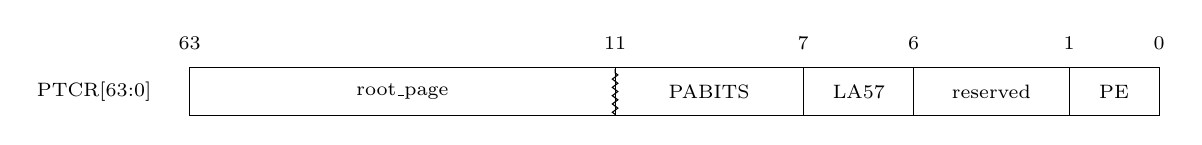
\begin{tikzpicture}[x=0.409in,y=0.24in,every node/.style={font=\scriptsize}]
\node[anchor=east] at (-0.35,0.50) {PTCR[63:0]};
\node[anchor=south] at (0.00,1.18) {63};
\node[anchor=south] at (5.20,1.18) {11};
\node[anchor=south] at (7.50,1.18) {7};
\node[anchor=south] at (8.85,1.18) {6};
\node[anchor=south] at (10.75,1.18) {1};
\node[anchor=south] at (11.85,1.18) {0};
\draw (0.00,0) rectangle (5.20,1);
\node at (2.60,0.50) {root\_page};
\draw[decorate,decoration={zigzag,amplitude=1.0pt,segment length=3pt}] (5.20,0.03) -- (5.20,0.97);
\draw (5.20,0) rectangle (7.50,1);
\node at (6.35,0.50) {PABITS};
\draw (7.50,0) rectangle (8.85,1);
\node at (8.18,0.50) {LA57};
\draw (8.85,0) rectangle (10.75,1);
\node at (9.80,0.50) {reserved};
\draw (10.75,0) rectangle (11.85,1);
\node at (11.30,0.50) {PE};
\end{tikzpicture}
\manualfigurecaption{PTCR Format}
\end{center}


@PTCR_FIELD_TABLE@

@PABITS_SELECTOR_TABLE@

\Needspace{1.35in}
\begin{center}\vspace{3pt}
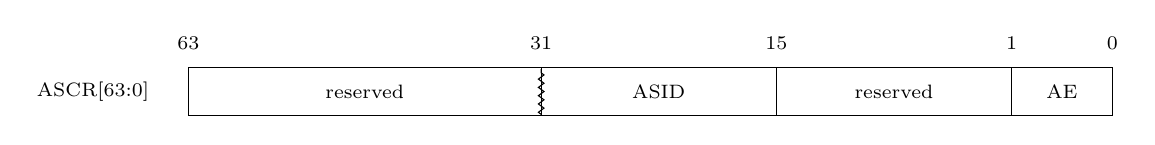
\begin{tikzpicture}[x=0.420in,y=0.24in,every node/.style={font=\scriptsize}]
\node[anchor=east] at (-0.35,0.50) {ASCR[63:0]};
\node[anchor=south] at (0.00,1.18) {63};
\node[anchor=south] at (4.20,1.18) {31};
\node[anchor=south] at (7.00,1.18) {15};
\node[anchor=south] at (9.80,1.18) {1};
\node[anchor=south] at (11.00,1.18) {0};
\draw (0.00,0) rectangle (4.20,1);
\node at (2.10,0.50) {reserved};
\draw[decorate,decoration={zigzag,amplitude=1.0pt,segment length=3pt}] (4.20,0.03) -- (4.20,0.97);
\draw (4.20,0) rectangle (7.00,1);
\node at (5.60,0.50) {ASID};
\draw (7.00,0) rectangle (9.80,1);
\node at (8.40,0.50) {reserved};
\draw (9.80,0) rectangle (11.00,1);
\node at (10.40,0.50) {AE};
\end{tikzpicture}
\manualfigurecaption{ASCR Format}
\end{center}


ASCR holds the current address-space identifier. SWPT Dn performs a page-table swap that clears ASCR.
SWPTA Dn, Dn performs a context-aware page-table swap: PTCR is updated, ASCR[31:16] is set from the
low 16 bits of the second data-register operand, and ASCR.AE is set.

@ASCR_FIELD_TABLE@

\Needspace{1.35in}
\begin{center}\vspace{3pt}
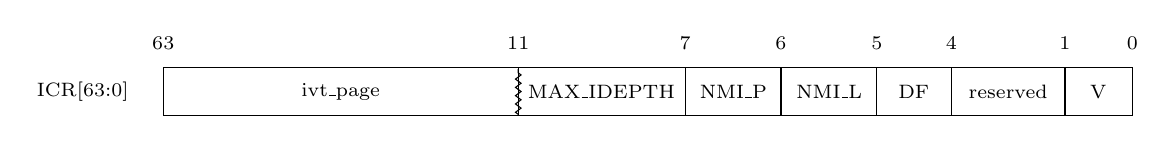
\begin{tikzpicture}[x=0.355in,y=0.24in,every node/.style={font=\scriptsize}]
\node[anchor=east] at (-0.35,0.50) {ICR[63:0]};
\node[anchor=south] at (0.00,1.18) {63};
\node[anchor=south] at (5.00,1.18) {11};
\node[anchor=south] at (7.35,1.18) {7};
\node[anchor=south] at (8.70,1.18) {6};
\node[anchor=south] at (10.05,1.18) {5};
\node[anchor=south] at (11.10,1.18) {4};
\node[anchor=south] at (12.70,1.18) {1};
\node[anchor=south] at (13.65,1.18) {0};
\draw (0.00,0) rectangle (5.00,1);
\node at (2.50,0.50) {ivt\_page};
\draw[decorate,decoration={zigzag,amplitude=1.0pt,segment length=3pt}] (5.00,0.03) -- (5.00,0.97);
\draw (5.00,0) rectangle (7.35,1);
\node at (6.17,0.50) {MAX\_IDEPTH};
\draw (7.35,0) rectangle (8.70,1);
\node at (8.03,0.50) {NMI\_P};
\draw (8.70,0) rectangle (10.05,1);
\node at (9.38,0.50) {NMI\_L};
\draw (10.05,0) rectangle (11.10,1);
\node at (10.57,0.50) {DF};
\draw (11.10,0) rectangle (12.70,1);
\node at (11.90,0.50) {reserved};
\draw (12.70,0) rectangle (13.65,1);
\node at (13.17,0.50) {V};
\end{tikzpicture}
\manualfigurecaption{ICR Format}
\end{center}


@ICR_FIELD_TABLE@

The detailed interrupt-vector and supervisor-entry frame layouts are described in the Exception Processing
Reference section.
